\section{Rutherford-Streuversuch}
%kurz das ziel dieses versuchsteiles ansprechen, damit keine zwei �berschriften direkt �bereinander stehen!
%bei schwierigeren versuchen kann auch der theoretische hintergrund erl�utert werden. (mit formeln, herleitungen und erkl�rungen)
In diesem Versuchsabschnitt soll die Streuung von $\alpha$-Strahlung an Goldfolie untersucht werden.

\subsection{Versuchsdurchf�hrung}
Die Streuung von $\alpha$-Teilchen an einer Goldfolie wird in einem Winkelbereich von -30$^\circ$ bis 30$^\circ$ in 5$^\circ$-Schritten untersucht. Neben der Goldfolie wird der Kollimator mit einer Spaltbreite von 1mm (\cite{anleitung}) eingesetzt. Die Streukammer wird auf 35 $\pm$ 3 mbar evakuiert. Die Messdaten werden mit dem Computer aufgenommen. F�r jeden Winkel wurde f�r einen Zeitraum von 180 $\pm$ 1 s gemessen. Die aufgenommen Histogramme werden mit der Poissonverteilung gefittet, da Zufallsvariablen, die die Anzahl von Ereignissen, die in einem gegebenen Zeitintervall Auftreten, darstellen, poissonverteilt sind (Beispiel im Anhang). Der Fehler des Winkels wurde mit 2$^\circ$ angenommen. Die so bestimmten Z�hlraten werden mit Gleichung \ref{eqn:ruth} gefittet. Da das Winkelma� einen Offset besitzt, wird dies durch eine additive Konstante als Fitparameter ber�cksichtigt.

\begin{align}
\label{eqn:ruth}
f(x) = \frac{A}{sin^4 \left[ \frac{(x-B)}{2} \right]}
\end{align}

\subsection{Auswertung}
In Abbildung \ref{fig:rutherford_gold} sind die Messdaten mit dem Fit der Rutherfordstreuformel zu sehen. Die Rutherfordstreuuformel wurde nach Gleichung \ref{eqn:ruth} gefittet. Dabei ergaben sich f�r den Fit die Werte in Tabelle \ref{tab:fit_gold_ruth}.

\begin{figure}[H]
	\centering
  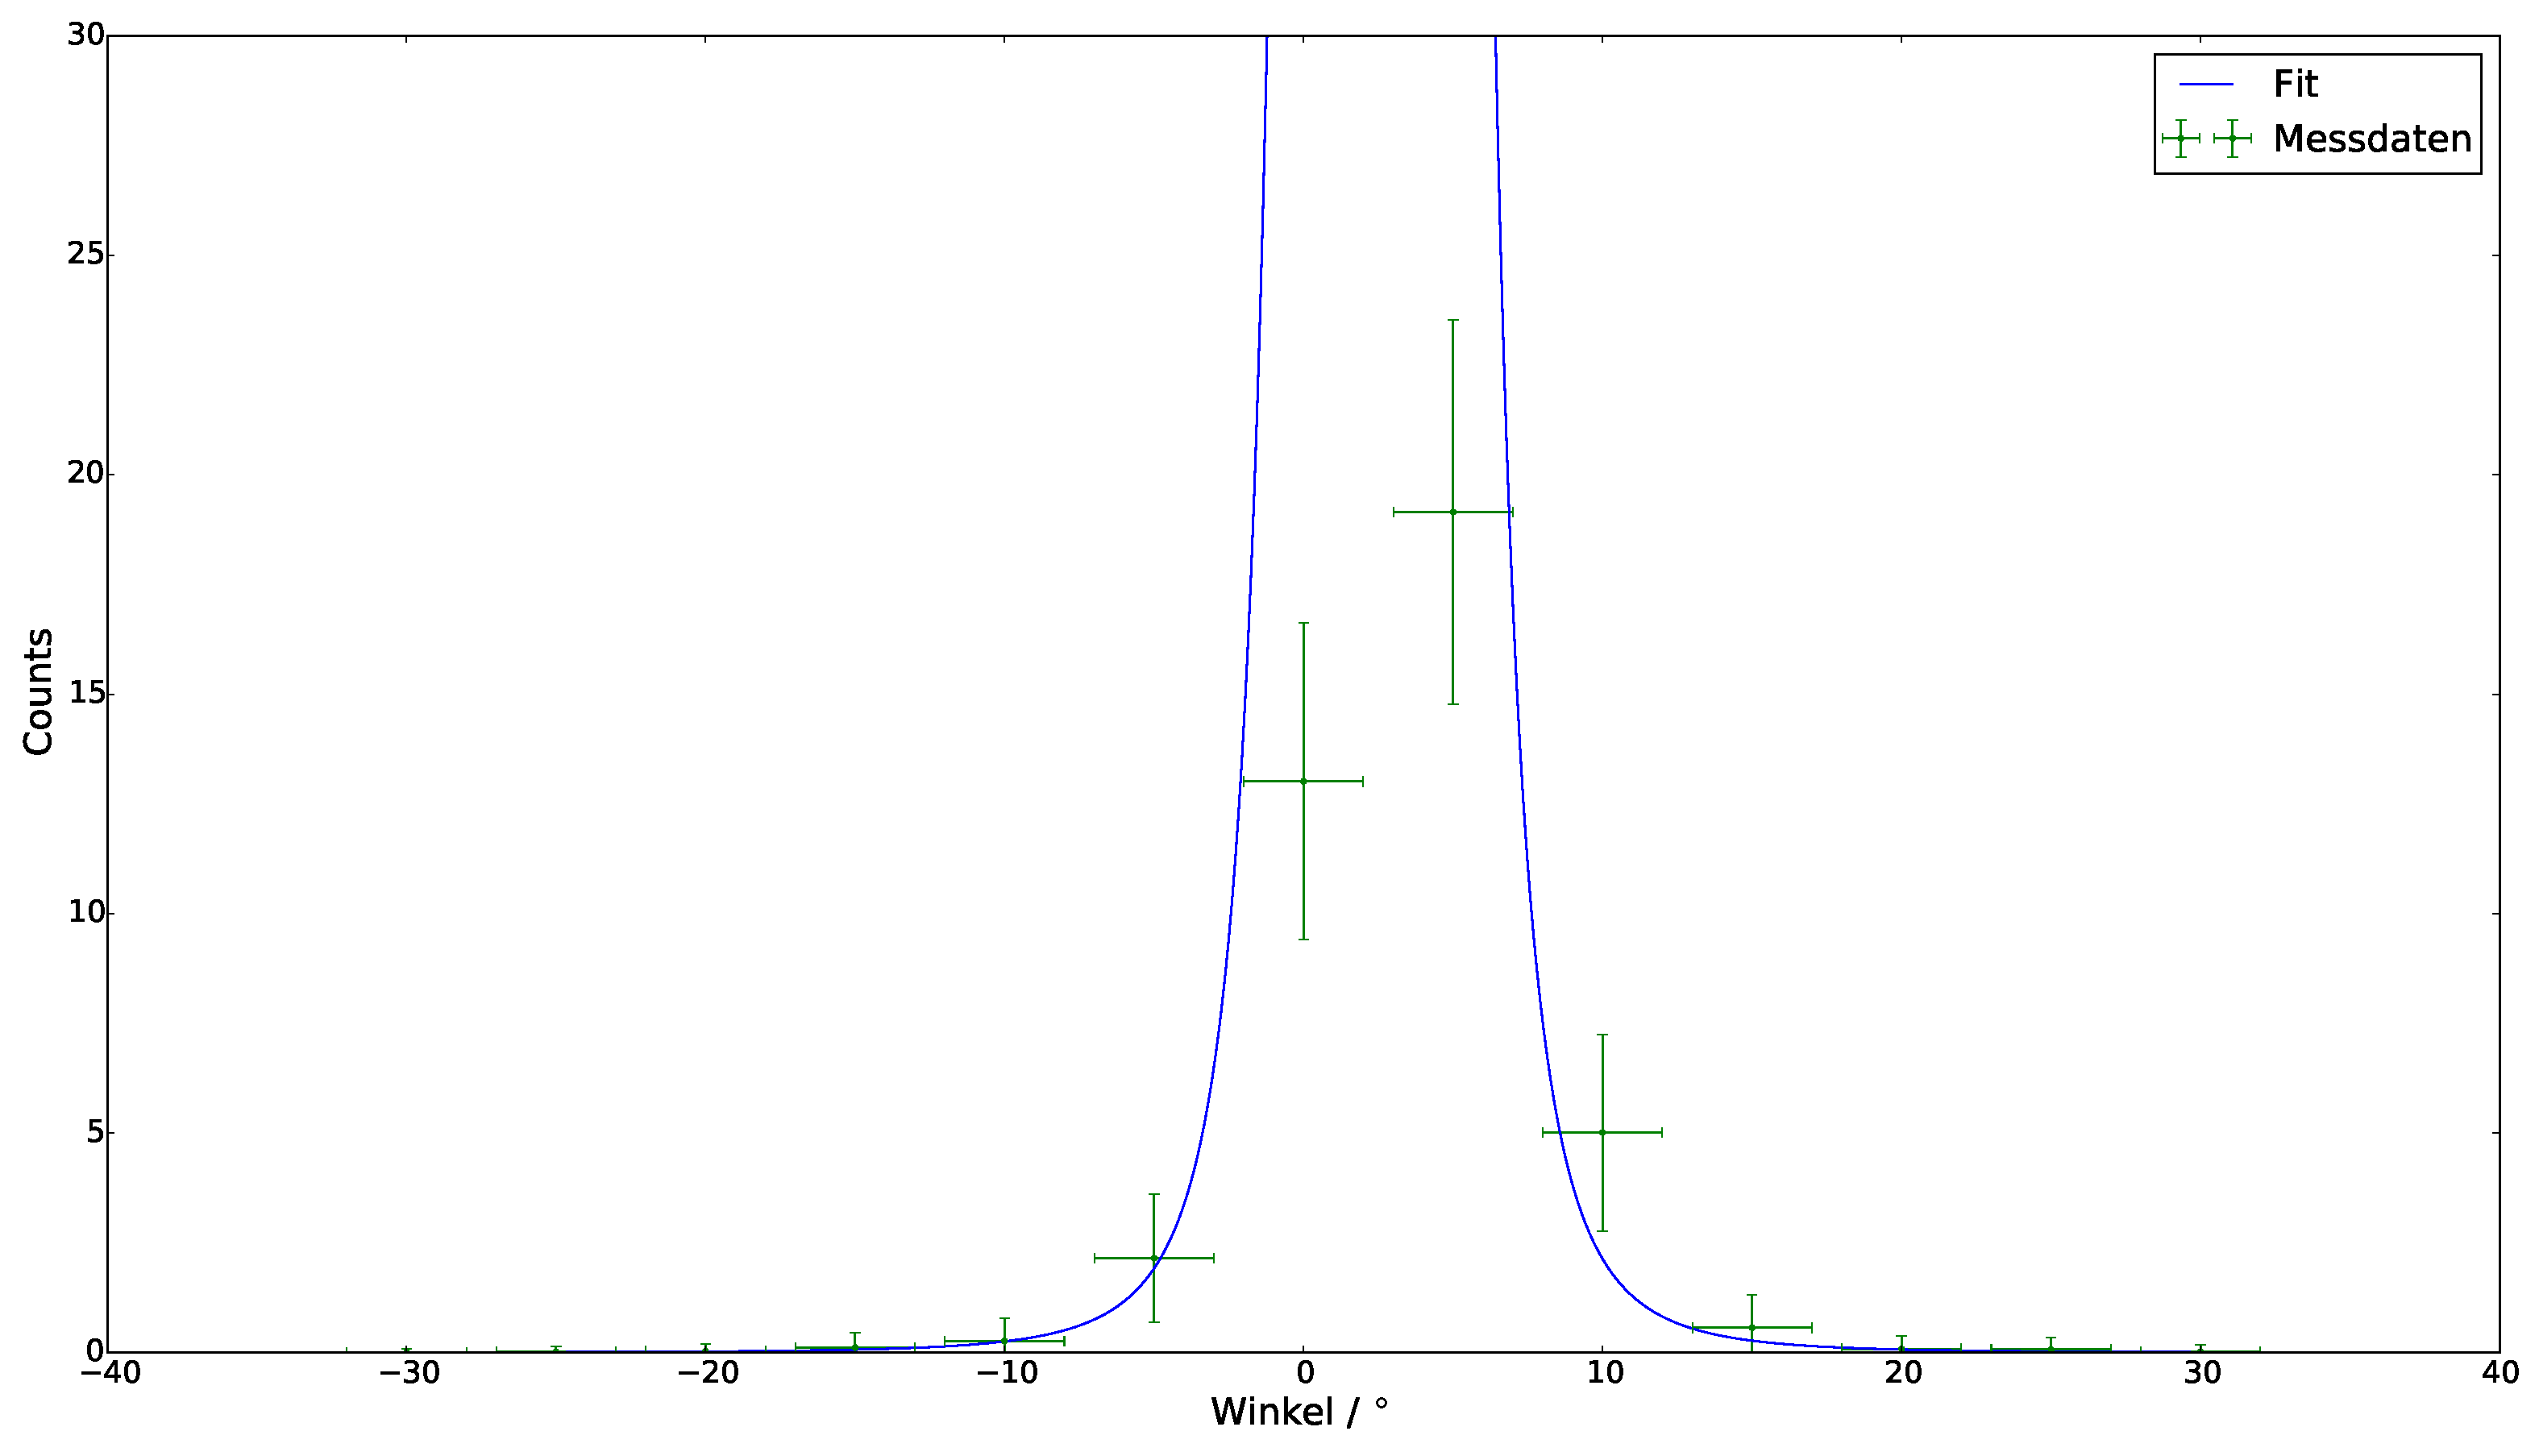
\includegraphics[scale=0.33]{rutherford_messung.pdf}
	\caption{Es sind die Messdaten aus der Streuung von $\alpha$-Strahlung an Gold zu sehen. Die Messdaten wurden mit  Gleichung \ref{eqn:ruth} gefittet, dabei ergab sich ein $\chi_{red}^2$ von 2,48.}
	\label{fig:rutherford_gold}
\end{figure}

\begin{table}[H]
\centering
\caption{Fitparamter f�r die Goldfolie nach Gleichung \ref{eqn:ruth}}
\label{tab:fit_gold_ruth}
\begin{tabular}{|c|c|}
\hline Paramter & Wert \\ 
\hline A/[barn] & 0,00037 $\pm$ 0,00002 \\ 
\hline B/$^\circ$ & 2,62 $\pm$ 0,05 \\ 
\hline $\chi_{red}^2$ & 2,48 \\ 
\hline 
\end{tabular} 
\end{table}


Der Fit passt optisch gut zu den Daten, auch wenn das $\chi_{red}^2$ nur einen Wert von 2,48 hat.